\documentclass[11pt]{article}

\usepackage{fullpage}
\usepackage{amsmath}
\usepackage{amssymb}
\usepackage{graphicx}

\parindent 0pt
\parskip 7pt

\title{CamScan}

\author{David Storch \\
	   Sam Birch \\
	   Michelle Micallef \\
	   Stylianos Anagnostopoulos}
\date{14 May 2011}

\begin{document}

\maketitle

\centering

\includegraphics[scale=0.4]{CamscanLogo}
\flushleft

\section*{What is CamScan?}

CamScan is a desktop application for converting images of printed content---taken with a personal camera, web cam, or smart phone---into usable documents. Users can import their images into CamScan's library, and let CamScan convert a group of related images into a searchable and selectable multipage PDF.

\section*{What can CamScan do?}

Automated corner finding and optical character recognition (OCR) comprise the core of CamScan's functionality. When a document is imported, CamScan uses automated corner finding to crop and rotate the image. At the same time, text extracted from the image via OCR makes the document searchable and selectable. Despite all of its automation, CamScan also allows the user to manually adjust image properties so as to produce the best final product.

\section*{Screenshots}

\subsection*{Edit Mode}

In \textbf{edit mode}, the user can manually choose cropping, rotation, and perspective adjustment. This is accomplished by allowing the user to choose the locations of the four corners of the document. There is also an interface at the bottom on the screen for correcting color and contrast of the image.

\centering
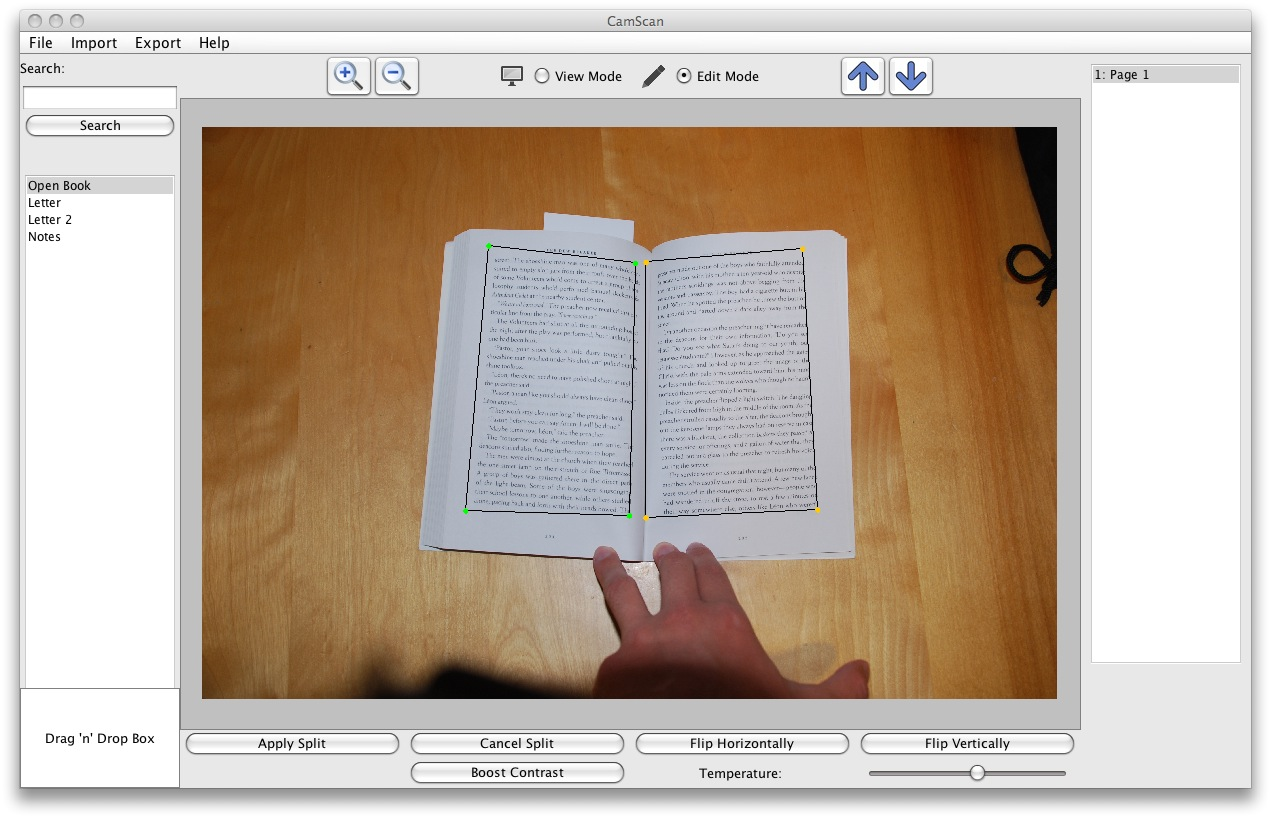
\includegraphics[scale=0.3]{editmode}
\flushleft

\subsection*{View Mode}

In \textbf{view mode}, the results of the image processing can be inspected. When a document is imported, view mode will appear, displaying the results of CamScan's image processing algorithm. The user can then switch to edit mode in order to make any necessary changes

\centering
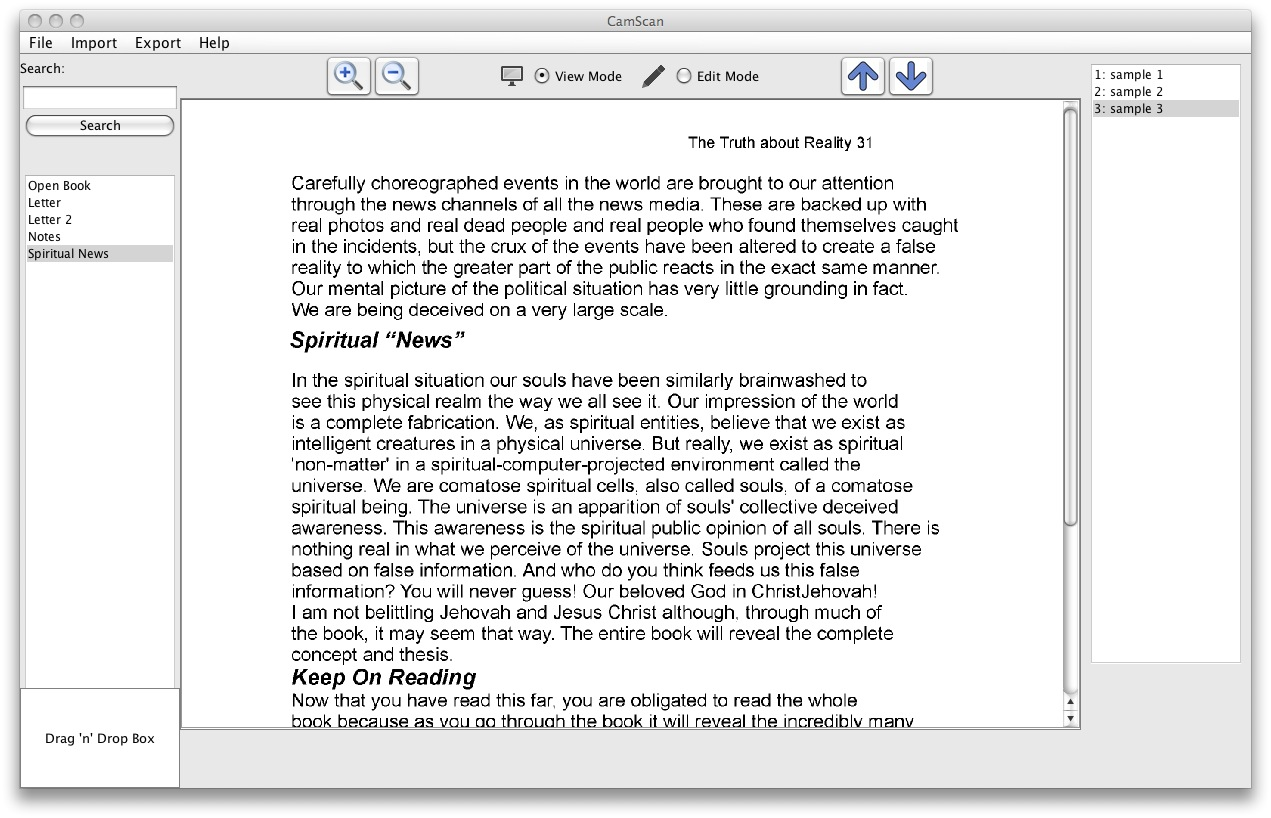
\includegraphics[scale=0.3]{viewmode}
\flushleft

\subsection*{Search Results}

The screenshot below shows the \textbf{search results} panel. Search hits are displayed as snippets of extracted OCR text. Selecting a result and clicking the "Go to Result" button navigates to the page from which the text was extracted.

\centering
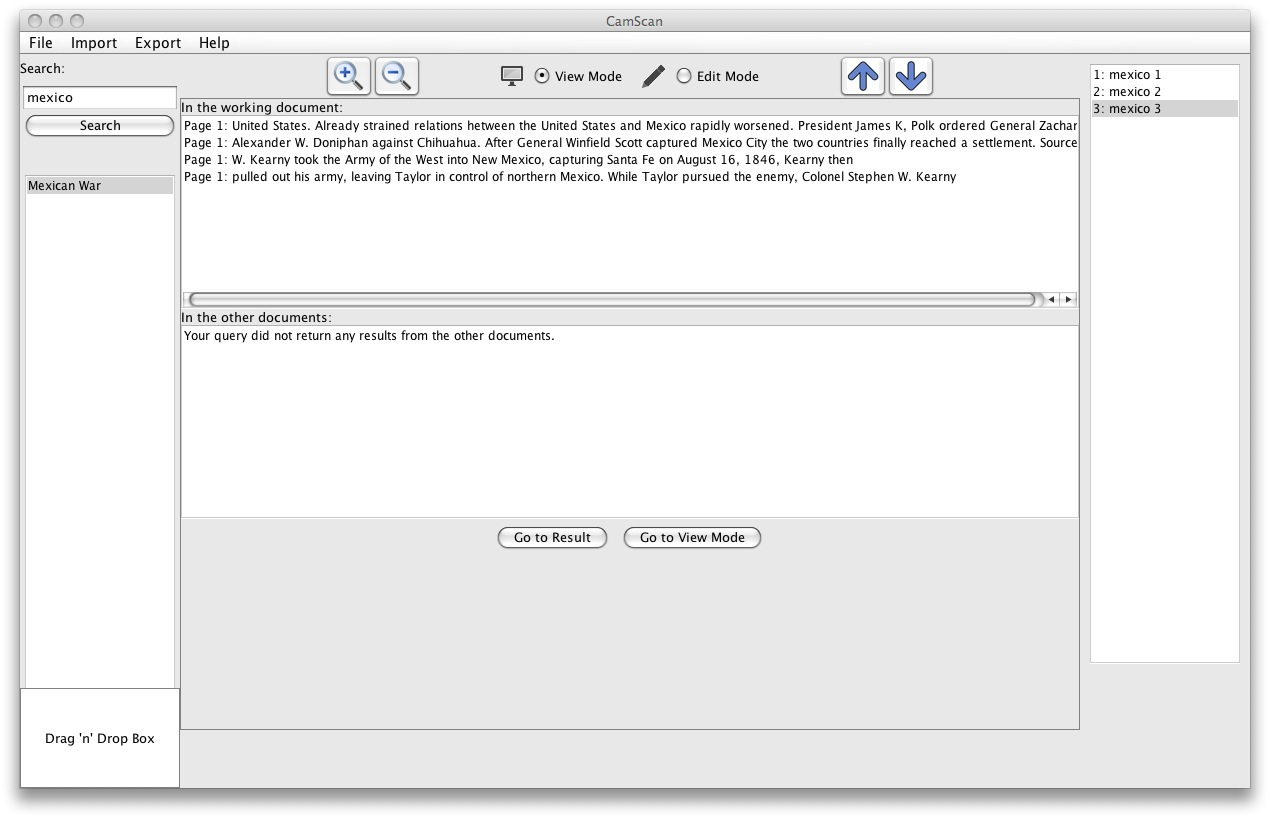
\includegraphics[scale=0.3]{searchresults}
\flushleft

\end{document}